\documentclass{article}
\usepackage[utf8]{inputenc}
\usepackage{tikz}
\usetikzlibrary{calc}
\usepackage{float}
\usepackage{graphicx}
\usepackage{listings}
\usepackage{karnaugh-map}
\title{Assignment 9 (GATE, EC2018,18)}
\author{SIKANDER KATHAT }
\date{25 December 2020}

\begin{document}

\maketitle

\section{ Question  18 MUX diagram }
\begin{figure}[!ht]
\centering
{
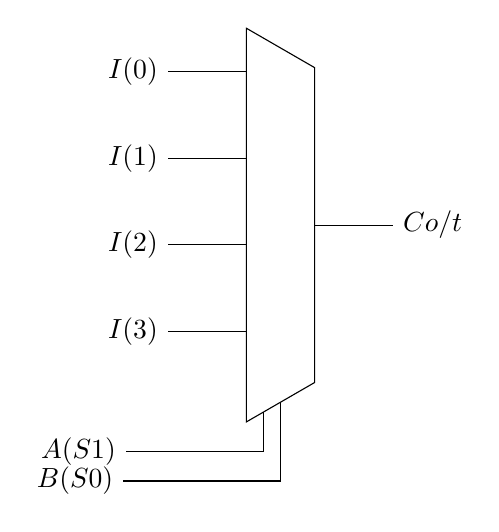
\begin{tikzpicture}
\draw (0,0)coordinate (O)--++(30:1)coordinate (P)--++(90:4)coordinate (Q)--++(150:1)coordinate (R)--cycle;
\draw($(P)!0.5!(Q)$)--++(0:1)node[right]{$Co/t$};
\draw($(O)!0.5!(P)$)--++(-90:1)--++(180:2)node[left]{$B(S0)$};
\draw($(O)!0.25!(P)$)--++(-90:0.5)--++(180:1.75)node[left]{$A(S1)$};
\foreach\y/\t in {0.1/(0),0.3/(1),0.5/(2),0.7/(3)} {
\draw ($(R)!\y*1.1!(O)$)--++(180:1)node[left]{$I\t$};}
\end{tikzpicture}

}
\caption{question MUX diagram}
\label{MUX diagram)}
\end{figure}

\section{Question 18}
A 4:1 multiplexer is to be used for generating the output carry of a full adder. A and B are the bits to be added while C(in) is the input carry and Co/t is the output carry. A and B are to be used as select bits with A being more significant select bit.

Which one of the following statement correctly describes the choice of signals to be connected to the inputs I(0), I(1), I(2) and I(3) so that the output is Co/t?

\begin{enumerate}
    \item$I(0)=0,I(1)=C(in),I(2)=C(in),I(3)=1$
    \item$I(0)=1,I(1)=C(in),I(2)=C(in),I(3)=1$
    \item$I(0)=C(in),I(1)=0,I(2)=1,I(3)=C(in)$
    \item$I(0)=0,I(1)=C(in),I(2)=1,I(3)=C(in)$
\end{enumerate}

\section{Solution}
\begin{table}[!ht]
{
\begin{tabular}{|l|l|l|l|l|}
\hline
A & B & C(in) & Sum(S) & Co/t \\ \hline
0 & 0 & 0     & 0      & 0    \\
0 & 0 & 1     & 1      & 0    \\
0 & 1 & 0     & 1      & 0    \\ 
0 & 1 & 1     & 0      & 1    \\
1 & 0 & 0     & 1      & 0    \\
1 & 0 & 1     & 0      & 1    \\
1 & 1 & 0     & 0      & 1    \\
1 & 1 & 1     & 1      & 1    \\ \hline
\end{tabular}

}
\caption{TRUTH TABLE}
\label{table}
\end{table}


\begin{figure}[!ht]
\centering
{
\begin{karnaugh-map}[4][2][1][][]
    \maxterms{0,3,5,6}
    \minterms{1,2,4,7}
    \implicant{1}{1}
    \implicant{2}{2}
    \implicant{4}{4}
    \implicant{7}{7}
    % note: position for start of \draw is (0, Y) where Y is
    % the Y size(number of cells high) in this case Y=2
    \draw[color=black, ultra thin] (0, 2) --
    node [pos=1, above right, anchor=south west] {$BC(in)$} % YOU CAN CHANGE NAME OF VAR HERE, THE $X$ IS USED FOR ITALICS
    node [pos=1, below left, anchor=north east] {$A$} % SAME FOR THIS
    ++(135:1);
        
    \end{karnaugh-map}

}
\caption{k-map for Sum(S)}
\label{kmap Sum(S)}
\end{figure}


    
    Boolean expression for Sum(S)-
    
    S=A$\overline{B}$ $\overline{C(in)}$ + $\overline{A}$ $\overline{B}$ C(in) + $\overline{A}$ B $\overline{C(in)}$ + ABC(in)
\newpage

\begin{figure}[!ht]
\centering
{
\begin{karnaugh-map}[4][2][1][][]
    \maxterms{0,1,2,4}
    \minterms{3,5,6,7}
    \implicant{3}{7}
    \implicant{5}{7}
    \implicant{7}{6}
    % note: position for start of \draw is (0, Y) where Y is
    % the Y size(number of cells high) in this case Y=2
    \draw[color=black, ultra thin] (0, 2) --
    node [pos=1, above right, anchor=south west] {$BC(in)$} % YOU CAN CHANGE NAME OF VAR HERE, THE $X$ IS USED FOR ITALICS
    node [pos=1, below left, anchor=north east] {$A$} % SAME FOR THIS
    ++(135:1);
        
    \end{karnaugh-map}

}
\caption{k-map for Co/t}
\label{kmap Co/t}
\end{figure}
 
 Boolean expression for Co/t-

Co/t= BC(in) + AB + AC(in)

\begin{table}[!ht]
\centering
{
\begin{tabular}{|l|l|l|} \hline
A & B & C o/t  \\ \hline
0 & 0 & 0      \\
0 & 1 & C(in)  \\
1 & 0 & C(in)  \\
1 & 1 & 1      \\ \hline
\end{tabular}



}
\caption{TRUTH TABLE for Co/t to be output}
\label{table 1 }
\end{table}
So, by the truth table for Co/t to be output,
we get 


{I(0)=0, I(1)= C(in), I(2)= C(in) and I(3)= 1}
\end{document};


